\section{Thesis objective and outline}
\subsection{Towards an innovative and AI-based methodology for controlling infectious disease in livestock farming from sensor observations}

Managing and controlling infectious animal diseases within livestock farming involves understanding and intervening within a highly complex system. This complexity arises from intrinsic parameters—such as pathogen strains and specific farming practices—as well as extrinsic parameters, notably detection methodologies and control measures, which are inherently variable over time. Compared to conventional control strategies, artificial intelligence (AI) has emerged as a particularly promising approach for conceptualizing epidemic dynamics, modeling their progression, and anticipating their evolution through simulations (Ezanno et al., 2021). Such simulations enable, at minimum, the evaluation and comparison of various disease management scenarios, and facilitate the creation of decision-support tools (DSTs) developed collaboratively with stakeholders such as farmers, veterinarians, animal science specialists, and public decision-makers (Ezanno et al., 2018).

The current period of agricultural digitalization further strengthens the integration of stakeholders with these DSTs, particularly through the emergence of AI-driven tools capable of constructing zootechnical descriptors that traditionally represented a significant manual workload for farm operators. Within the broader scope of precision agriculture, there has been significant development and deployment of sensor technologies designed to continuously monitor physiological variables at the individual animal scale, as well as environmental conditions at the farm level. These sensors aim to generate short-term alerts (on the order of hours or days) related to critical stages of animal life cycles (such as parturition or estrus), animal welfare, and even, in crop farming contexts, risks associated with weather conditions (thermal or hydric stress) or ecological threats like pest invasions (Liakos et al., 2018).

Nevertheless, particularly in animal health contexts concerning infectious diseases, sensor-generated alerts tend to lack specificity, resulting in a high incidence of false positives. Such false alarms impose substantial cognitive burdens on farm operators, who consequently either disregard these alerts due to their perceived irrelevance or initiate unnecessary and excessive interventions. Hence, designing innovative methodologies that, despite the inherent lack of specificity in sensor alerts, can provide precise and actionable recommendations over longer and more human-compatible planning horizons (spanning several days or weeks), remains an open research question. It is precisely this unresolved challenge that this thesis seeks to address.

Consequently, the core research question guiding this thesis is: "How can sensor observations be effectively employed to study infectious diseases and support informed decision-making?"

\begin{figure}
  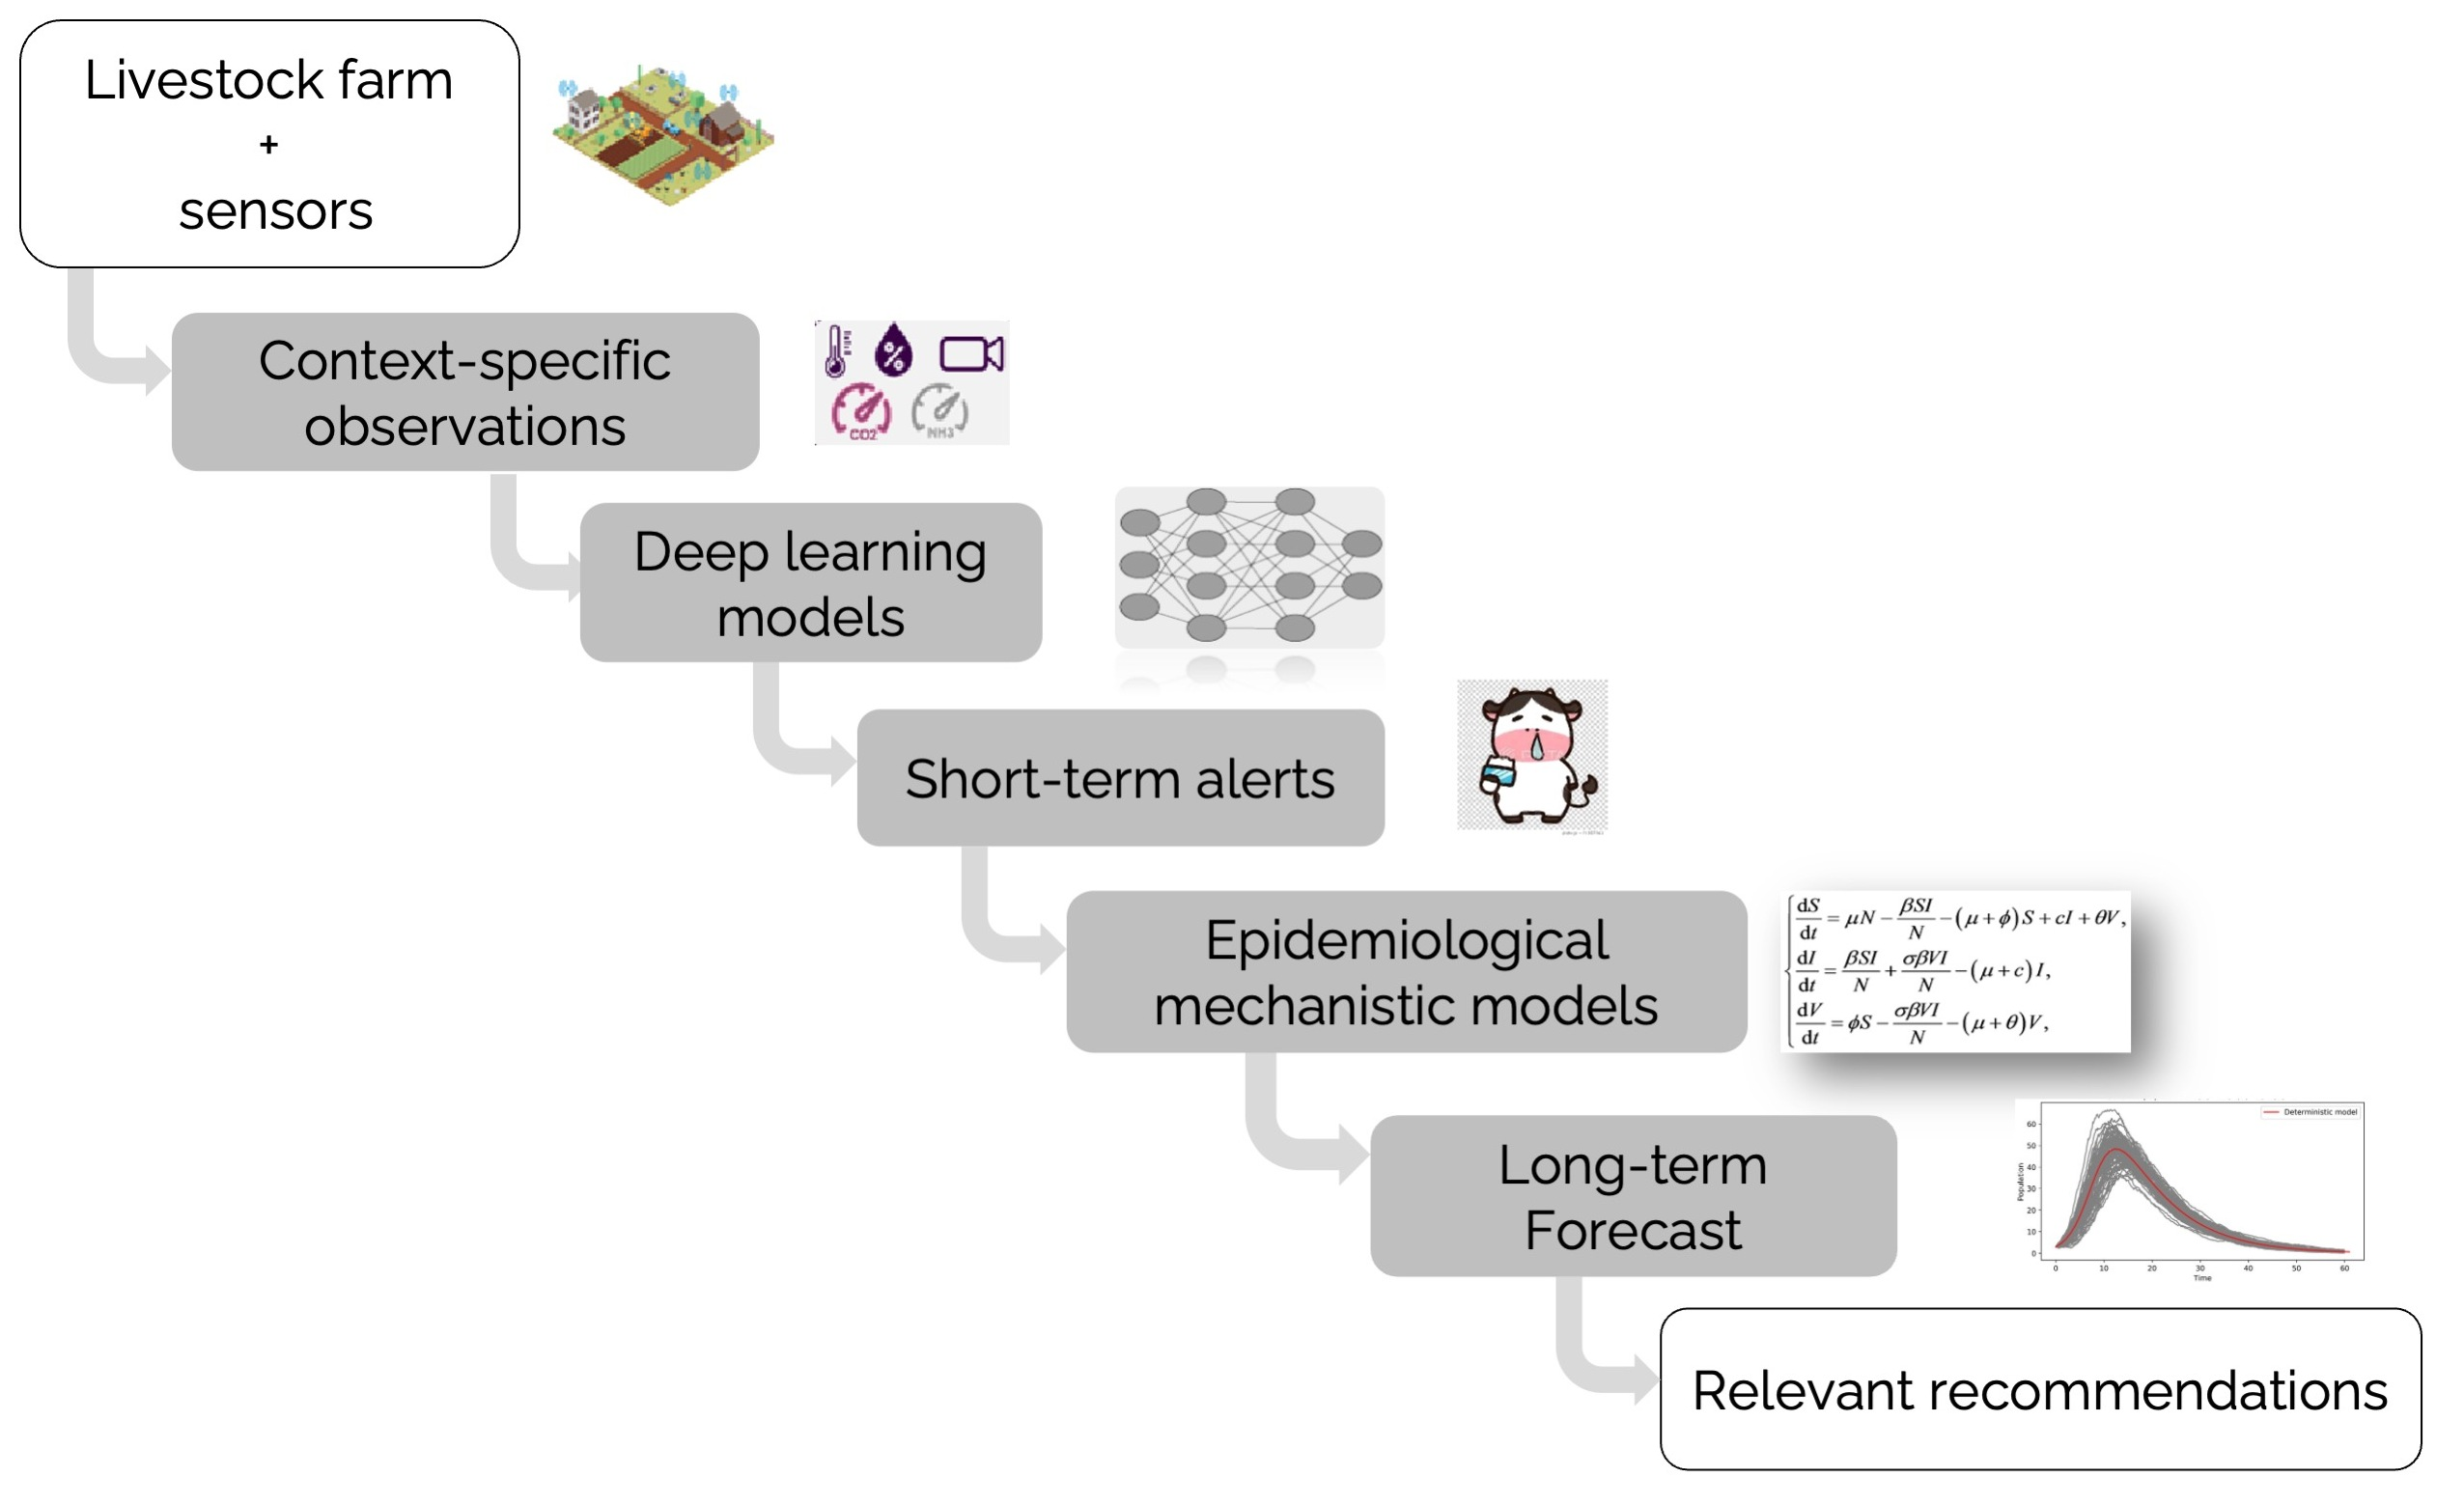
\includegraphics[width=\linewidth]{figures/chap1/chap1-outline.jpg}
  \caption{How can sensor observations be effectively employed to study infectious diseases and support informed decision-making?}
  \label{fig:chap1-outline}
\end{figure}
\newpage

Our primary hypothesis (Fig \ref{fig:chap1-outline}) posits that the optimal scientific approach to address contemporary quantitative challenges in animal health involves the integration of diverse artificial intelligence methodologies. In this thesis, we explore the complementarity between deep learning models and mechanistic epidemiological models. This integrative strategy leverages the extensive representation capabilities, multi-level analysis, and interdisciplinary expressivity of mechanistic epidemiological models while capitalizing on deep learning’s robust data-mining capabilities. This fusion aims to achieve better integration of real-world observational data (derived from sensors, farmers, and veterinarians) with disease predictions across multiple temporal scales—ranging from short-term (days) to medium and long-term (weeks or months).


\subsection{Use-case: Bovine Respiratory Diseases in young beef cattle sector}

Bovine Respiratory Disease (BRD) represents the foremost animal health concern in cattle feedlots, negatively impacting animal welfare, economic performance, and public health through excessive antimicrobial use (Taylor et al., 2010). BRD significantly reduces animal growth rates and productivity, resulting in increased veterinary and medicinal expenses, as well as higher mortality rates—averaging approximately 3\% (Engler et al., 2014). It is also the primary reason antibiotics are administered in cattle production, affecting roughly 20\% of fattening cattle (Assié et al., 2009).

The etiology of BRD is multifactorial (fig \ref{fig:chap1-BRDetiology}), arising from complex interactions among intrinsic and extrinsic factors. Intrinsically, animal susceptibility is influenced by breed, immunity, and simultaneous infection by multiple pathogens, notably Mannheimia haemolytica, Pasteurella multocida, and Bovine Respiratory Syncytial Virus (BRSV), whose interactions are not yet fully understood (Cusack \& Lean, 2003; Duff \& Galyean, 2007). Extrinsic risk factors—such as stressful transportation conditions, herd density, feed management, housing conditions, biosecurity protocols, and climatic conditions—also strongly influence disease occurrence and severity (Cusack \& Lean, 2003; Duff \& Galyean, 2007). Together, these intrinsic and extrinsic complexities severely limit the reliability of BRD prognosis, control strategies, and disease modeling.


\begin{figure}[h]
  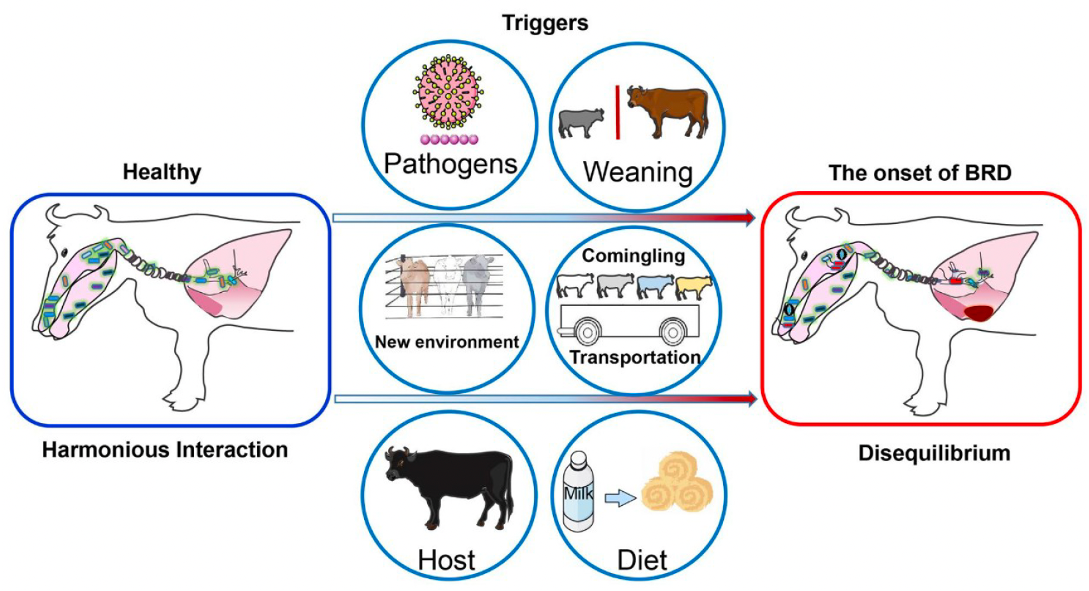
\includegraphics[width=\linewidth]{figures/chap1/BRD etiology.png}
  \caption{BRD etiology. From Jio-anmin et al., 2022. Burden in animal welfare, antimicrobial use and economic costs.}
  \label{fig:chap1-BRDetiology}
\end{figure}

Diagnosing BRD is particularly challenging due to non-specific clinical presentations such as cough, nasal discharge, hyperthermia, anorexia, lethargy, and impaired growth—symptoms overlapping with many other diseases (Cusack \& Lean, 2003; Griffin, 2010). Traditional visual detection based on behavioural appraisal is limited, displaying low sensitivity (62\%) and specificity (approximately 63\%), thereby resulting in frequent misdiagnoses (false positives) or delays in detection (White \& Renter, 2009; Weary et al., 2009). Moreover, cattle often mask early clinical symptoms due to inherent prey behaviour, complicating timely and accurate identification of infected animals (Griffin, 2010). Additionally, limited veterinary expertise in rural areas of France further exacerbates accurate detection.

Recent advances in precision livestock farming (Allain et al., 2014; Berckmans, 2014) have enabled continuous monitoring of animal health through sensor technologies such as accelerometers, microphones, thermometers, and cameras, measuring bio-signals indicative of BRD (e.g., body temperature, behavioural patterns, and respiratory sounds) (Guatteo et al., 2015). Timsit et al. (2011) previously demonstrated that about 73\% of hyperthermia episodes were associated with BRD, suggesting temperature-based monitoring's potential diagnostic utility. More recently, Concordet et al. (2022) developed logistic regression models using sensor data (collar, pedometer, intra-ruminal bolus), achieving sensitivity and specificity rates of approximately 75\% and 76\%, respectively, capable of predicting BRD clinical signs up to 24 hours in advance. Similarly, Ramezani et al. (2022) evaluated accelerometer-based ear-tag sensors detecting behavioural changes (activity, inactivity, rumination), demonstrating significant differences between healthy and diseased calves, although further validation in larger cohorts remains necessary.

Despite promising early detection results, most sensor-based studies remain limited by reliance on traditional machine learning models incapable of robust forecasting, hindering their predictive utility for scenarios that differ significantly from observed data. This limitation restricts their capacity to support evidence-based management and informed control interventions effectively, as complete observation of BRD dynamics in field conditions is ethically and practically unfeasible. One study even proposed that further studies with higher number of diseased animals are necessary to improve their performance. 

Complementary to sensor-based approaches, mechanistic epidemiological modelling has emerged as a promising solution to overcome observational limitations. Picault et al. (2022) conducted an in silico modelling study identifying potential sensor-based management strategies. However, these mechanistic models were primarily calibrated from existing veterinary literature rather than empirical sensor data, resulting in uncertainties regarding their practical and explanatory utility in real-world veterinary scenarios. Furthermore, such modelling often involves invasive and expensive sensor technologies, underscoring the necessity of exploring alternative, non-invasive, cost-effective sensor modalities (e.g., audio, video, image analysis) for broader deployment.

Addressing these critical limitations, this thesis, collaboratively developed by INRAE, Adventiel, and myself :), seeks to develop innovative artificial intelligence methodologies specifically tailored for BRD diagnostics and prognostics, yet adaptable to other livestock or plant epidemiological contexts. By integrating deep learning with mechanistic epidemiological modelling, this work explicitly aims to enhance the interpretability, accuracy, and predictive robustness of sensor-derived observations (see Fig \ref{fig:chap1-outline}). The resulting methodologies aims to minimize inappropriate antimicrobial usage, improve animal welfare, reduce economic losses, and support long-term, evidence-based decision-making in precision livestock farming.


% \textcolor{red}{dans les discussions pour le chapitre 1, il faudrait que j'indique que je notre sensibilité fait raccord avec ce qui est dit dans la littérature en utilisant uniquement les signes cliniques. Mais en quantifiant l'incertitude du modèle et celle contenue dans les données, on a pu améliorer la précision générale et en plus filtrer les observations considérée comme bruyantes.}


\subsection{Originality of this thesis}

\subsubsection{synergy of various domain expertise}
% In this subsection, I want to explain the thesis CIFRE, with the mixture of domain expertise: epidemiological mechanistic modelling, statistical inference approaches, computer vision and deep learning, hardware and software engineering Mais également la collaboration avec les vétos. Préciser que c'est une thèse cifre (ce que peut apporter/ et les gains en retours pour adventiel: les côté applicatif, igepp (deep), Dynamo (mécaniste, inférence...). It is original to have as many different domain experts come together to work on one subject right ?

In France, a CIFRE (Convention Industrielle de Formation par la Recherche) thesis is a program that fosters collaboration between a doctoral candidate, a company, and a public research laboratory. this initiative allows companies to hire a doctoral student to conduct research aligned with their strategic interests, while the student simultaneously works towards their Ph.D. The research is supervised jointly by the company's scientific advisor and an academic supervisor from the affiliated research laboratory. This arrangement aims to strengthen public-private research partnerships and enhance innovation within companies.

Adventiel is a French digital services company specializing in the agricultural and agri-food sectors. They assist businesses in their digital transformation by designing innovative, tailor-made technological solutions. Their expertise includes web and mobile application development, data science, artificial intelligence, software publishing, hosting, and IT management. 

INRAE (the French national research institute for agriculture, food, and environment) is a public research organization. As the world's leading research institute in its fields, INRAE focuses on generating scientific knowledge, fostering innovation, and informing public policies to address global challenges such as climate change, biodiversity loss, and food security.

Ces rapprochements méthodologiques entre santé animale et santé végétale sont une priorité forte d’INRAE depuis plusieurs années et font également écho aux orientations du développement des activités de R\&D d’Adventiel. 

Cette thèse s'est appuyée sur les acquis méthodologiques et applicatifs des partenaires académiques et privé :
\begin{enumerate}
    \item Une nouvelle approche de modélisation générique combinant représentation des connaissances et système multi-agents multi-niveaux pour générer des modèles épidémiologiques spécialisés : l’approche EMULSION [Picault et al 2019b], développée dans l’équipe DYNAMO de BIOEPAR (INRAE) ; A Domain-Specific Language (DSL) is a specialized computer language tailored to address problems within a specific domain, offering a higher level of abstraction optimized for that particular area.  
    
    Framework EMULSION is intended for modellers in epidemiology, to help them design, simulate, and revise complex mechanistic stochastic models, without having to write or rewrite huge amounts of code. It comes with a Domain-Specific Language to represent all components of epidemiological models (assumptions, model structure, parameters…) in an explicit, intelligible and revisable way, and thus facilitate interactions with other scientists (biologists, veterinarians, economists…) throughout the modelling process. EMULSION models are automatically processed by a modular simulation engine, which, if needed, can also incorporate small code add-ons for representing very specific features of a model. Models can use classical modelling paradigms (compartments, individual-based models, metapopulations) and multiple scales (from individuals to metapopulations). Emulsion has been very usefull in this thesis notably for running and easily adapting mechanistic models to one desire, for instance I had to sometimes change the output of the mechanistic model, and even without understanding everything, EMULSION programming language made it easier to identify and adapt the code as necessary.

    \item Un ensemble de travaux autour de la modélisation des BRD mobilisant plusieurs équipes de BIOEPAR [Picault et al 2019a] et garantissant une expertise sur les aspects vétérinaires, épidémiologiques, immunologies et socio-économiques de ces maladies; Parmis lesquel on retrouve le premier mécaniste  pour étudier et controller les BRD développé dans EMULSION. Ce modèle notamment mécaniste a été ré-utilisé dans les travaux de cette thèse afin de répondre à certaines de nos questions scientifiques (voir partie 1.3.4).

    \item Un ensemble de projets d’apprentissage profond, développé au sein d’Adventiel, qui construisent à partir de données hétérogènes (images, vidéos et sons) des indicateurs de bien-être animal. Adventiel a également fourni le nécessaire en terme de hardware et configuration des serveurs de stockage des données qui ont été collectés durant la thèse. Dans le cadre de projets, des modèles de deep learning (archictectures confidentielles) ont été développés pour analyser le comportement de bovin sur des vidéos, ou encore détectés des anomalies sonores dans des données acoustiques. Donc en plus de ramené de la connaissance en deep, Adventiel dispose également de serveurs qui ont permis de stocker les données qui ont été collectées durant cette thèse. 

    \item Plusieurs méthodes et expertises développées au sein de l'équipe Démécologie d'IGEPP (INRAE) ont pu être transféré à notre problématique. The objective of the Démécologie team is to understand and predict the impact of disruptions on epidemic dynamics at the population level. In the context of human activity management, these disruptions can occur in space, such as habitat heterogeneity from within individual plots to entire landscapes. They can also manifest over time, through intra- and inter-seasonal life cycles. Additionally, they may affect life traits, including phenotypic plasticity and reproductive modes, as well as inherited information, such as polymorphism and variations in genetic recombination across genomes. Their statistical modelling approach, notably when looking at inverse modelling, uncertainty modelling through Bayesian inference methods and "Experimentation governed by modelling and theory" has been a great help for answering some scientific questions of this thesis.
\end{enumerate}


\subsubsection{Dataset}

L’ensemble de ces travaux ont pu fournir un socle solide sur lequel développer des méthodes originales. les différents corpus de données utilisés pendant la thèse proviennent des synergies avec des projets académiques en cours :
\begin{itemize}
    \item le projet européen H2020 DECIDE dont l'unité de recherhe BIOEPAR est partenaire, qui s’attache à comprendre diverses maladies respiratoires et digestives dans plusieurs espèces d’animaux de production ;
    \item la chaire de télémédecine vétérinaire d'Oniris, qui permettra d’équiper divers élevages;
    \item le projet Carnot France Futur Élevage SEPTIME (BIOEPAR + Idele, institut de l’élevage) qui vise à concevoir un outil d’aide à la décision combinant un modèle mécaniste des BRD et des informations de capteurs en temps réel, afin que les situations théoriques décrites dans le modèle puissent mettre à jour leurs projections en fonction de la situation observée sur le terrain. ; 
\end{itemize}

\begin{figure}[h]
  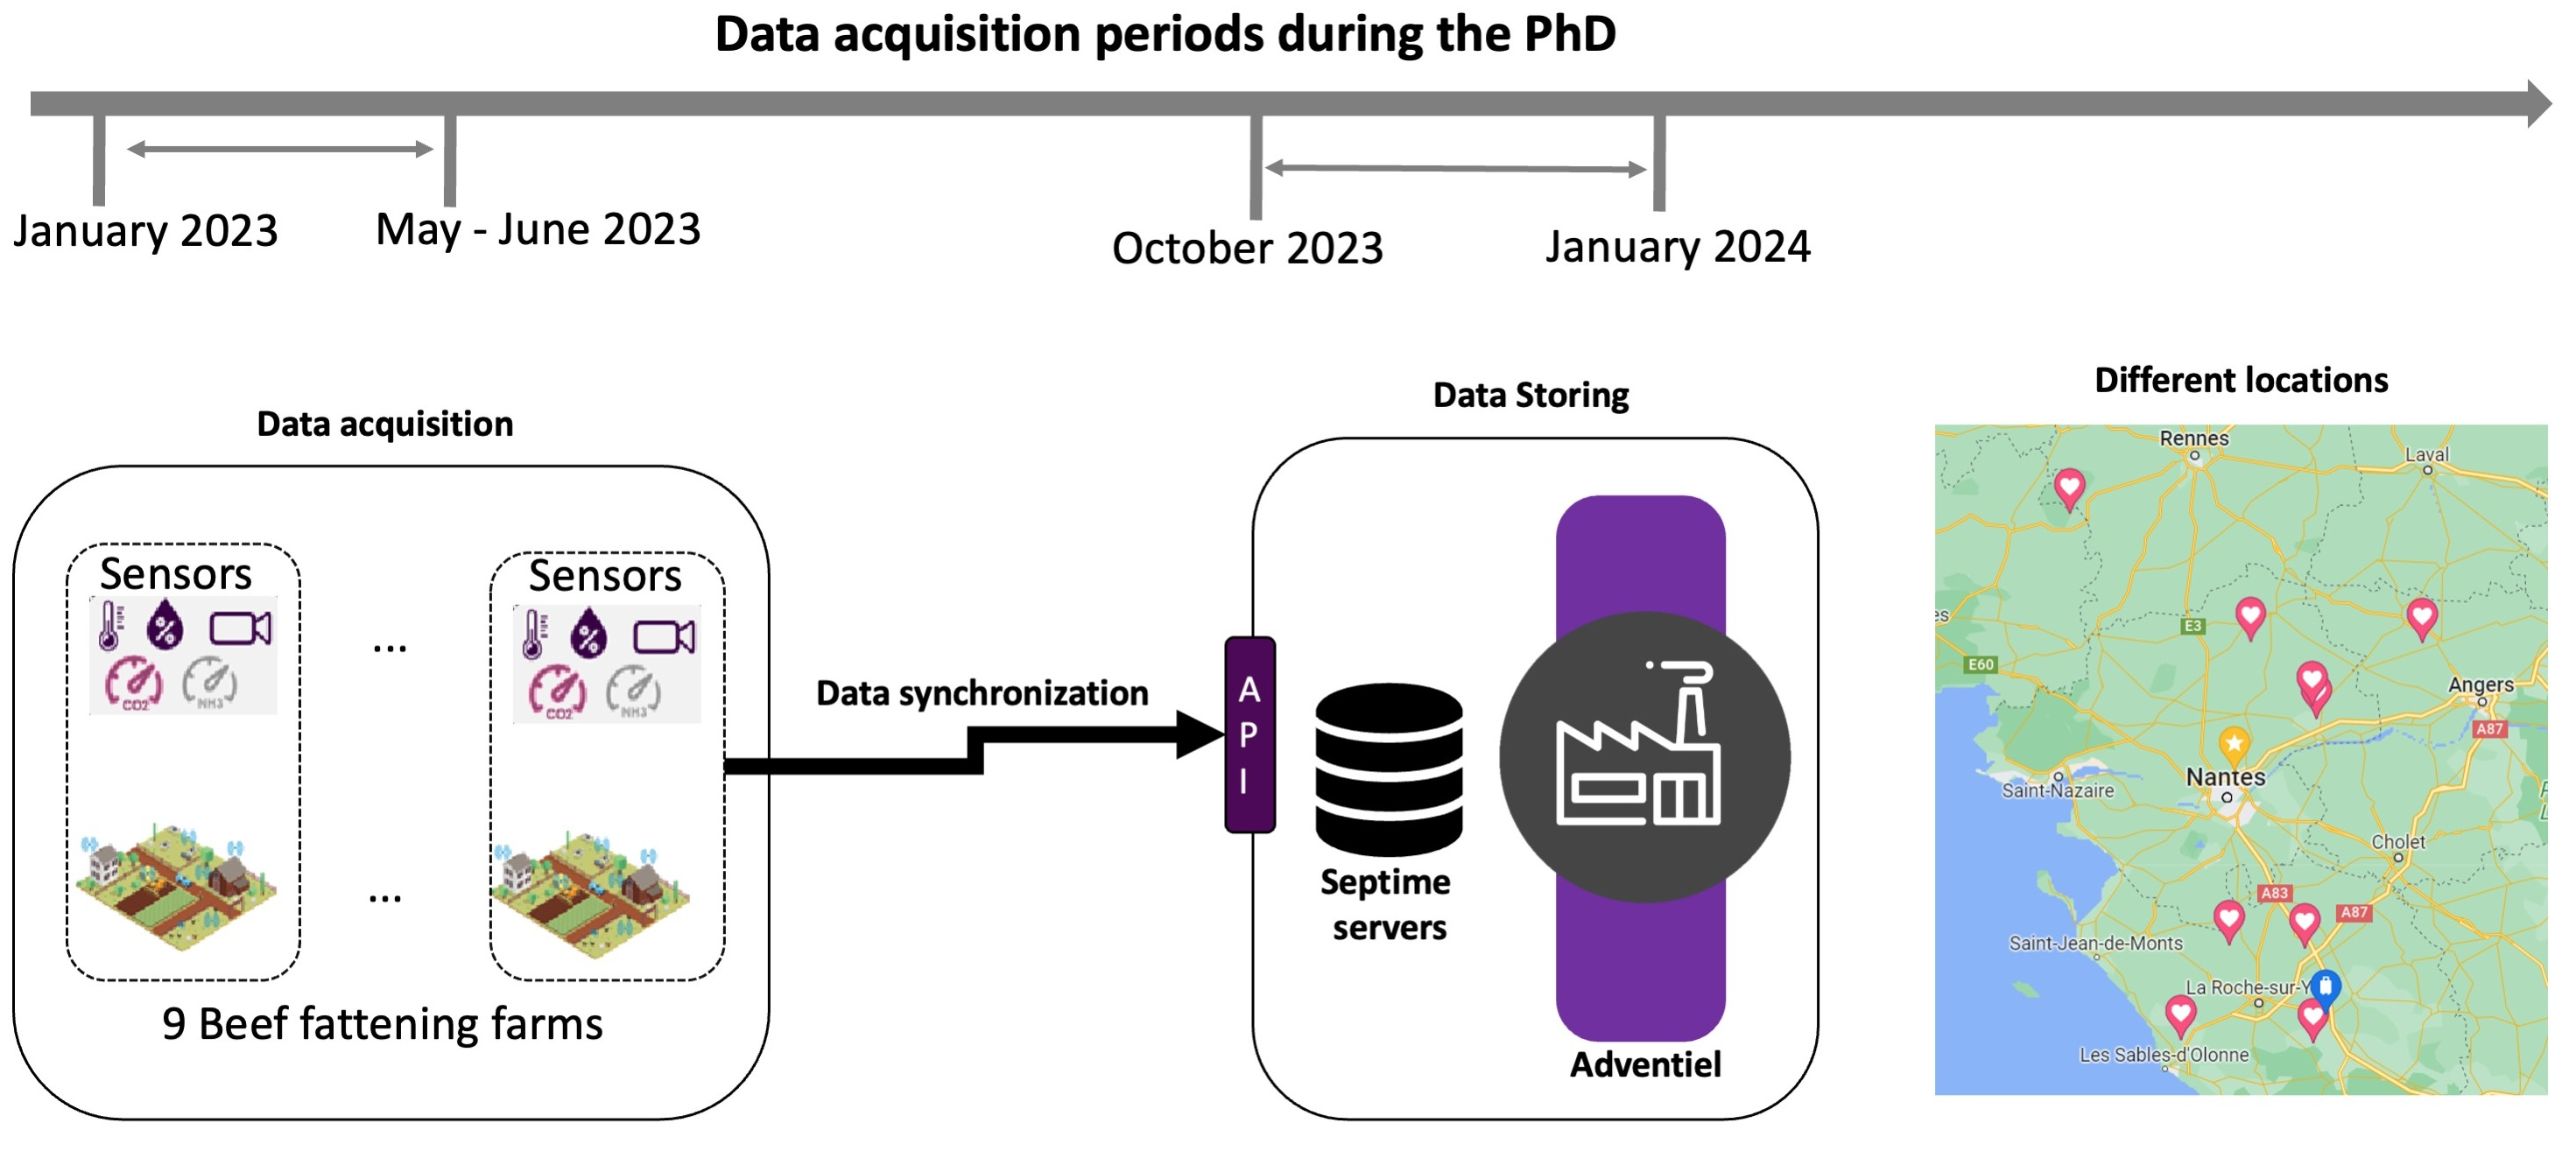
\includegraphics[width=\linewidth]{figures/chap1/data collection.jpg}
  \caption{Data collection}
  \label{fig:chap1-DataCollection}
\end{figure}

Through the Septime Project, we gathered a comprehensive observational dataset collected specifically to study BRD. [describe the data experimental protocol with these elements]
\begin{itemize}
    \item 9 farms beef fattening farms in France
    \item Each farm having up to 3 batches containing each 5 to 12 animals
    \item 78\% of bovine were of race Charolaise (known for having a white fur, and expressing  easily visible clinical symptoms)
    \item I set-up various sensors in the 9 farms: per farm, i set-up one camera that records 5 mins worth of video everyday from 9 a.m till 6 p.m, one microphone that synhcronize the acoustic recording with the video surveillance footage of the camera, one environmental sensor that measures the temperature, humidity, $CO_2$ and $NH_3$
    \item A veterinarian (Maud also part of the Septime project) would come often (every 2 days) to perform examinations on the animals. The study was conducted during 30 days after arrival at batch.
    \item veterinarians examinations both performed clinical and biological examinations of the animals. biological examinations consisted in blood samples for deep analysis through laboratory testing on pcr test on nasal swabs to identify the presence of pathogens in upper aerial respiratory track. clinical examinations could either be a  examination where they assess clinical signs such as (fatigue, ocular discharge, nasal discharge, rectal temperature). (an example copy of the assessment table can be found in the appendix) 
    \item As an additional sensor, veterinarians also had the possibility to scan the lung of all the animals through an ultrasound scanner. This was performed at different observation dates (day 0, day 5, day 14, day 21, day 28) these dates were also taken according to the availability of the veterinarian. 
    \item Apart from setting-up the sensors inside the farms, I also coded and configured the communication between the sensors in the farm and the storage server located at Adventiel.
\end{itemize}


This dataset, comprising multi-modal sensor data, lung ultrasound videos, and expert veterinary examinations has helped simultaneously address fundamental scientific questions and practical agricultural needs for potentially informing innovative and practical decision-support tools.
 

\subsubsection{About the methodological approach and contributions}

% \paragraph{Methodology: diagnosis and prognosis expertise}

The goal of this PhD is to create new knowledge on the complementarities between deep learning modelling and epidemiological mechanistic model to effectively employ sensor observations in order to study and control infectious diseases in livestock farming. In the work of this thesis, we particularly focused on study and controlling the spread of BRD in the beef cattle farm. For that, we set-up an original program constituted of actors with interdisciplinary expertise (deep learning model, statistical inference, epidemiological mechanistic modelling, veterinarian knowledge), with the hardware (servers) and sensors. The thesis structure progresses methodologically across three chapters:


% Les fronts de science traités pendant cette thèse seront donc (i) le développement d'algorithmes d'apprentissage profond spatio-temporelle et/ou ensembliste pour la construction de descripteurs santé [Mahmud et al 2021], (ii) l'étude de la fiabilité de ces descripteurs pour le couplage au modèle mécaniste (e.g. biais, variance, cohérence) et enfin (iii) l'étude des capacités prédictives des modèles mécanistes informés par de tels indicateurs sur des horizons épidémiques longs.


Chapter 2 - Foundational structures:


This chapter assesses independently the performance of the deep learning model in automating the BRD diagnosis from lung ultrasound video data, reaching an accuracy of 72\%. It also evaluates a stochastic mechanistic epidemiological model parametrized by veterinarian-provided clinical observations, confirming its utility for robust long-term BRD prognosis, albeit with moderate calibration precision due to observational data scarcity and inherent uncertainties in observations. Demonstrating feasibility of deep learning diagnosis from limited, real-world sensor data and creating an original annotated dataset of lung ultrasound observations, forming an empirical foundation for further research. This directly addresses scientific questions 1 and 2.

\begin{enumerate}
    \item To what extent can deep learning reliably automate short-term diagnosis using limited, and context-specific observational data from sensors, such as lung ultrasounds videos ? Our objective is to evaluate the extent to which deep learning architectures can autonomously derive high-level semantic representations from lung ultrasound videos.
    
    \item How can mechanistic epidemiological models be parametrized using empirical veterinary observations to provide accurate long-term prognosis for BRD ?  we investigate whether empirical veterinary assessments considered ground truth, collected at limited temporal intervals and sparse frequency, can effectively parametrize a mechanistic epidemiological model to reliably predict BRD dynamics. 

    \item To what extent can we reliably differentiate between multiple pathogen-specific mechanistic models of BRD, solely based on symptomatic observations ? we introduce a numerical approach aimed at distinguishing among competing BRD mechanistic epidemiological models based exclusively on observed symptomatic trajectories. 

    \item Does the distinction and identification of the most likely pathogen-specific mechanistic model significantly improve practical decision-making outcomes ? we explicitly incorporate an economic dimension into our analysis by integrating pathogen-specific model predictions into a bio-economic framework. This enables us to quantify practical benefits for the farmers. 

    \item To what extent can automated short-term diagnostics derived from limited sensor observations effectively inform and specify a mechanistic epidemiological model for long-term disease prognosis ? we develop an approach that leverages short-term, sensor-derived diagnostics obtained from limited Lung Ultrasound (LUS) video data to inform parameter calibration in an epidemiological model for BRD. 

    \item How can intrinsic uncertainties inherent in sensor-derived diagnostic data, especially noisy observations such as Lung Ultrasound (LUS) videos, be explicitly quantified and incorporated into mechanistic models to ensure a more robust and trustworthy prognostic prediction ? Given the intrinsic uncertainty and noisiness of real-world LUS videos, exacerbated by animal movement and image acquisition limitations, this work explicitly addresses the quantification and integration of these uncertainties into the diagnostic and prognostic pipeline.
\end{enumerate}





This thesis proposes an original methodological framework that combines deep learning and mechanistic epidemiological modelling, with articulated contributions:
\begin{itemize}
    \item Automated Diagnosis from limited and Noisy Observational Data from a sensor: Demonstrating the feasibility and robustness of deep learning (CNN-RNN) approaches to automatically diagnose Bovine Respiratory Disease (BRD) using unstructured, context-specific sensor data (lung ultrasound videos), achieving reliable diagnostic accuracy despite limited data availability.
    \item automated prognosis from limited observations: establishing a robust methodological framework to independently parametrize and calibrate stochastic mechanistic models directly from empirical veterinary observations collected on-farm. This significantly enhances the identifiability, predictive accuracy, and practical relevance of long-term epidemiological forecasts for BRD management.
    \item Introducing clear numerical methods (Approximate Bayesian Computation with multinomial logistic regression) for reliably selecting among multiple competing mechanistic epidemiological models based solely on symptomatic observational data. This enables accurate pathogen-specific model identification, substantially reducing antibiotic misuse and improving farm economic outcomes.
    \item Structured Deep Mechanistic Modelling for Adaptive Knowledge Integration: proposing and validating a structured hybrid modelling pipeline (Bayesian Deep Mechanistic approach) explicitly linking deep learning-generated diagnostic information to mechanistic epidemiological prognosis. This novel approach grounds theoretical epidemiological knowledge directly within realistic, unstructured sensor observations, thereby providing a comprehensive, adaptive methodological baseline.
    \item Proxy Robustness and Explicit Uncertainty Quantification: Enhancing hybrid model reliability by explicitly quantifying and incorporating uncertainties inherent in noisy sensor observations (through Bayesian methods). This methodological improvement significantly reduces diagnostic and prognostic errors, thereby mitigating negative impacts arising from observational uncertainty.
    \item Modularity and Methodological Flexibility: Emphasizing methodological modularity, this thesis demonstrates how domain experts (veterinarians, deep learning specialists, mechanistic modellers) can independently develop, maintain, retrain, and adapt each modelling component. Such modularity contrasts favourably with tightly integrated approaches (e.g., Neural Differential Equations or Physics-Informed Neural Networks), offering significant advantages in interpretability, scalability, ease of use, reduced data requirements, and enhanced generalizability across diverse epidemiological contexts.
\end{itemize}


The thesis structure progresses methodologically across three chapters:

Chapter 2 - Foundational structures: independent diagnosis and prognosis expertise. 
This chapter assesses independently the performance of the deep learning model in automating the BRD diagnosis from lung ultrasound video data, reaching an accuracy of 72\%. It also evaluates a stochastic mechanistic epidemiological model parametrized by veterinarian-provided clinical observations, confirming its utility for robust long-term BRD prognosis, albeit with moderate calibration precision due to observational data scarcity and inherent uncertainties in observations. Demonstrating feasibility of deep learning diagnosis from limited, real-world sensor data and creating an original annotated dataset of lung ultrasound observations, forming an empirical foundation for further research. This directly addresses scientific questions 1 and 2.

Chapter 3 - Structural synergism – Selecting appropriate mechanistic prognosis experts. This chapter addresses a critical methodological gap: distinguishing among multiple valid mechanistic models, each suited to distinct pathogen-specific scenarios. Employing synthetic outbreak scenarios and a Bayesian inference framework, the chapter demonstrates how symptomatic dynamics can reliably inform pathogen-model identification. Integrating this approach with bioeconomic evaluations, we quantify the tangible benefits (improved net profits and reduced antimicrobial usage) resulting from pathogen-informed antibiotic treatment decisions. This directly addresses scientific question 3.

Chapter 4 - A deep mechanistic approach.  This chapter proposes a Bayesian deep mechanistic approach explicitly integrating observational uncertainties into both diagnostic and prognostic stages. Employing Monte Carlo Dropout (MCD) within the deep learning model, we quantify uncertainty in lung ultrasound observations and propagate it into mechanistic model calibration through uncertainty-weighted inference. This approach reduces diagnostic uncertainty (error rate reduced from 39\% to 27.2\% RRMSE), significantly enhancing model robustness and reliability for practical livestock management scenarios. This integration enhances decision-making robustness and aligns closely with real-world constraints where sensor observations are often noisy or incomplete. thus explicitly addressing scientific questions 4 and 5 by demonstrating how uncertainty-informed hybrid methodologies enhance practical livestock management reliability.

General discussion - The final section synthesizes the findings across all chapters, critically evaluating the methodological approaches, their strengths and limitations, and the broader implications of the results. Recommendations for future research and applications are also discussed, highlighting the potential for scalability and interdisciplinary adaptation.
